\section{Množiny}

\begin{definition}[Množina]\label{def:mnozina}
\emph{Množina} je súbor objektov, nazývaných \emph{prvkami množiny}.
Fakt, že objekt $x$ je prvkom množiny $A$ značíme takto:
$$x \in A$$
Ak objekt $x$ nepatrí do množiny $A$, značíme to takto:
$$x \notin A$$
\end{definition}

Množiny môžu byť konečné alebo nekonečné.
Konečnú množinu môžeme špecifikovať prostým vymenovaním jej prvkov takto:
$$A = \{1, \text{slon}, \{2\}\}$$
Platí $1 \in A$, slon $\in$ $A$.
Zrejme $4 \notin A$ mačka $\notin$ $A$.

\begin{question}
Platí $2 \in A$?
Odpoveď: nie.
\end{question}

Ale ak si niekto myslí, že áno, musí si myslieť, že objekt 2 je rovný niektorému z objektov, ktoré patria do množiny $A$.
Pravdepodobne si myslí, že
$$2 = \{2\}$$
To však nie je pravda: 2 nie je množina a \{2\} je množina a teda tieto dva objekty nemôžu byť rovné, pretože rovnaké objekty majú rovnaké vlastnosti.
Príkladom nekonečnej množiny je množina všetkých prirodzených čísel
$$\mathbb{N}=\{0,1,2,3,4,...\}$$
Všimnime si, že $0 \in \mathbb{N}$;
je možné, že na iných prednáškach to bude konvencia $0 \notin \mathbb{N}$.
Ďalšie množiny čísel, ktoré poznáte zo strednej školy, sú:
\begin{itemize}
    \item množina všetkých celých čísiel $\mathbb{Z}$
    \item množina všetkých racionálnych čísel $\mathbb{Q}$
    \item množina všetkých reálnych čísel $\mathbb{R}$.
\end{itemize}

\begin{definition}[Prázdna množina]
\emph{Prázdna množina} je množina, ktorá neobsahuje žiadny objekt. Prázdnu množinu značíme $\emptyset$.
\end{definition}

\begin{definition}[Podmnožina]
Hovoríme, že množina $B$ je \emph{podmnožinou} množiny $A$, ak pre každý prvok $x$ množiny $B$ platí, že $x \in A$.
Fakt, že $B$ je podmnožinou $A$ značíme
$$B \subseteq A$$
Ak $B$ nie je podmnožinou $A$, značíme $B \not\subseteq A$.
Vzťah $B \subseteq A$ sa volá \emph{inklúzia}.
\end{definition}

\noindent\textbf{Príklady:}
\begin{itemize}
    \item $A=\{1, \text{slon}, \{2\}\}$, potom
    \item $\{1, \text{slon}\} \subseteq A$
    \item $\{1, \{2\}\} \subseteq A$
    \item $\{1,3\} \not\subseteq A$, lebo $3 \in \{1,3\}$ a zároveň $3 \notin A$
    \item $\{2\} \not\subseteq A$, lebo $2 \in \{2\}$ a zároveň $2 \notin A$
\end{itemize}

\noindent V jazyku formálnej logiky $B \subseteq A$ zapisujeme takto:
%$$ (\forall x), x \in B \Rightarrow x \in A $$
%Pre všetky $x$ platí, že ak $x$ patrí do $B$, potom $x$ patrí do $A$.
\begin{center}
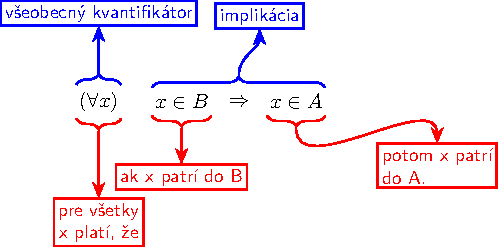
\includegraphics{figures/predn1_fig1.pdf}
\end{center}
\noindent Iný spôsob čítania tej istej formuly je tento:
%$$ (\forall x \in B), x \in A $$
%Pre všetky $x$ z množiny $B$ platí, že $x$ patrí do $A$.
\begin{center}
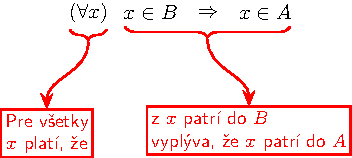
\includegraphics{figures/predn1_fig2.pdf}
\end{center}
Iný spôsob zápisu $B\subseteq A$ je tento
\begin{center}
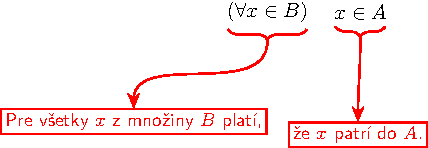
\includegraphics{figures/predn1_fig3.pdf}
\end{center}
Tieto symbolické zápisy sú logicky ekvivalentné, teda vyjadrujú rovnaký vzťah medzi množinami $B$ a $A$.
V tejto chvíli je dobré uvedomiť si, že prázdna množina je podmnožinou každej množiny.
Naozaj, ak by pre nejakú množinu $A$ platilo $\emptyset \not\subseteq A$, musel by existovať prvok $x$ množiny $\emptyset$ taký, že $x$ nepatrí do $A$.
Inak povedané, malo by platiť $x \in \emptyset$ a zároveň $x \notin A$;
to však nie je možné, pretože $x \in \emptyset$ neplatí pre žiadny objekt $x$.
Pri úvahách o vzťahu "byť podmnožinou" sme vlastne používali toto tvrdenie:

\begin{veta}
Nech $A, B$ sú množiny.
Potom $B \not\subseteq A$ práve vtedy, keď existuje $x \in B$ také, že $x \notin A$.
\end{veta}

\noindent V jazyku formálnej logiky:
%$$ (\exists x), x \in B \land x \notin A $$
%Existuje také $x$, že $x$ patrí do $B$ a zároveň $x$ nepatrí do $A$.
\begin{center}
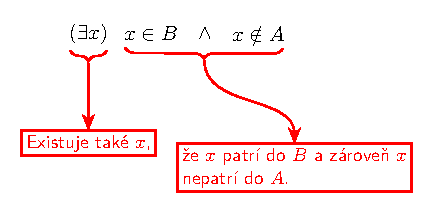
\includegraphics{figures/predn1_fig4.pdf}
\end{center}
Kedy sú dve množiny rovné?
Keďže množina je súbor objektov do nej patriacich, dve množiny sú rovné, ak obsahujú rovnaké prvky:
$$A = B \text{ práve vtedy, keď pre všetky objekty } x \text{ platí, že } x \in A \text{ práve vtedy, keď } x \in B.$$
Táto vlastnosť množín sa volá extenzionalita.
Z toho vyplýva nasledujúce tvrdenie:

\begin{veta}
Nech $A, B$ sú množiny. Potom $A=B$ práve vtedy, keď $A \subseteq B$ a zároveň $B \subseteq A$.
\end{veta}

Jeden zo spôsobov ako môžeme špecifikovať množinu je vydelenie z nejakej množiny pomocou výroku o prvkoch:
$$ \{x \in A \mid \text{výrok o } x\} $$
\textbf{Príklady:}
\begin{itemize}
    \item $\{x \in \mathbb{R} \mid x \ge 2\} = \langle 2, \infty)$
    \item $\{x \in \mathbb{R} \mid x > 3\} = (3, \infty)$
    \item $\{x \in \mathbb{R} \mid x \ge 4 \text{ a zároveň } x < 100\} = \langle 4, 100)$
    \item $\{x \in \mathbb{R} \mid x \ge 3 \text{ a zároveň } x < 2\} = \emptyset$
    \item $\{x \in \mathbb{R} \mid x^2 = 2\} = \{\sqrt{2}, -\sqrt{2}\}$
    \item $\{x \in \mathbb{N} \mid x^2 = 2\} = \emptyset$
    \item $\{n \in \mathbb{N} \mid (n+1) \text{ je prvočíslo}\} = \{1, 2, 4, 6, ...\}$
\end{itemize}

Podobný (ale významovo odlišný) zápis je
$$ \{ \text{výraz závislý od } x \mid x \in A \} $$
\textbf{Príklady:}
\begin{itemize}
    \item $\{n^2 \mid n \in \mathbb{N}\} = \{0, 1, 4, 9, 16, ...\}$
    \item $\{\sin(x) \mid x \in \mathbb{R}\} = \langle -1, 1 \rangle$
\end{itemize}

\subsection{Kardinalita množiny}
Počet prvkov konečnej množiny $A$ sa volá kardinalita $A$ a označujeme $|A|$.
\noindent\textbf{Príklady:}
\begin{itemize}
    \item $|\{1,7,8\}|=3$
    \item $|\emptyset|=0$
    \item $|\{\{4'4,2,3\}\}|= 1$
    \item $|\{\emptyset\}|=1$
\end{itemize}

\subsection{Operácie na množinách}
Ak $A, B$ sú množiny môžeme z nich vytvoriť inú množinu pomocou množinových operácií.
\begin{align*}
    A \cup B &= \{x \mid x \in A \text{ alebo } x \in B\} \quad \text{(zjednotenie množín A, B)} \\
    A \cap B &= \{x \mid x \in A \text{ a zároveň } x \in B\} \quad \text{(prienik množín A, B)} \\
    A \setminus B &= \{x \in A \mid x \notin B\} \quad \text{(rozdiel množín)}
\end{align*}

\noindent\textbf{Príklady:}
\begin{itemize}
    \item $\{1,2,3\} \cup \{2,3,4\} = \{1,2,3,4\}$
    \item $\{1,2,3\} \cap \{2,3,4\} = \{2,3\}$
    \item $\langle 2,4 \rangle \cap \langle 3,5 \rangle = \langle 3,4 \rangle$
    \item $\langle 2,3 \rangle \cap \langle 3,5 \rangle = \emptyset$
    \item $\langle 2,4 \rangle \cup \langle 3,5 \rangle = \langle 2,5 \rangle$
    \item $A \cap A = A \cup A = A$, pre všetky množiny $A$
    \item $\{1,2,3\} \setminus \{2,3,4\} = \{1\}$
    \item $\langle 2,4 \rangle \setminus \langle 3,5 \rangle = \langle 2,3)$
    \item $\mathbb{R} \setminus \mathbb{Q} = \text{iracionálne čísla}$
    \item $A \setminus A = \emptyset$, pre všetky množiny $A$
\end{itemize}

\subsection{Kartézsky/Priamy súčin množín}
Ak $a, b$ sú nejaké objekty, môžeme z nich vytvoriť objekt zvaný usporiadaná dvojica $(a, b)$. Dôležité je, že $(a,b) \neq (b,a)$, ak $a \neq b$.
V dvojici $(a,b)$, $a$ je prvá zložka a $b$ je druhá zložka.

\begin{definition}[Kartézsky súčin]
Nech $A, B$ sú množiny.
\emph{Kartézsky súčin} $A \times B$ je množina všetkých usporiadaných dvojíc $(a, b)$, kde $a \in A$ a $b \in B$.
Symbolicky: $A \times B = \{(a,b) \mid a \in A, b \in B\}$.
\end{definition}

\noindent\textbf{Príklady:}
\begin{itemize}
    \item $\{1,2\} \times \{3,4\} = \{(1,3), (1,4), (2,3), (2,4)\}$
    \item $\{1\} \times \{\square, \oplus\} = \{(1,\square), (1,\oplus)\}$
    \item $\{3,4\} \times \{1,2\} = \{(3,1), (3,2), (4,1), (4,2)\}$
\end{itemize}
Vidíme, že vo všeobecnosti nie je pravda, že $A \times B = B \times A$.
\begin{question}
Čo je $A \times \emptyset$?
\end{question}
$$ A \times \emptyset = \{(a,b) \mid a \in A, b \in \emptyset\} $$
Taký objekt $b$ neexistuje!
Teda $A \times \emptyset = \emptyset$ pre každú množinu $A$.
Nič nám nebráni vytvoriť kartézsky súčin $A \times A$: ak $A=\{1,2\}$, potom
$$A \times A = \{(1,1), (1,2), (2,1), (2,2)\}$$
Toto sa označuje aj $A^2$ -- druhá kartézska mocnina.
Analogicky ako pojem usporiadanej dvojice môžeme vytvoriť pojem usporiadanej trojice,
štvorice, $n$-tice, $n \in \mathbb{N}$.
\[
(a,b,c)\quad(a,b,c,d)\quad(a_1,\dots,a_n)
\]
Neformálne budeme na prednáškach používať
neexistujúce slovenské slovo ,,tica'' ak budem chcieť vyjadriť, že niečo je dvojica,
trojica, ..., ale pritom mi je jedno koľko zložiek má.
Toto je pokusom anglického
slova \emph{tuple}.
Pojem kartézskeho súčinu dvoch množín môžeme rozšíriť analogicky na viac množín:
\begin{align*}
    A \times B \times C &= \{(a,b,c) \mid a \in A, b \in B, c \in C\} \\
    A \times B \times C \times D &= \{(a,b,c,d) \mid a \in A, b \in B, c \in C, d \in D\}
\end{align*}
Na tomto predmete nás budú najmä zaujímať tieto množiny:
\begin{itemize}
    \item $\mathbb{R}^1 = \mathbb{R}$
    \item $\mathbb{R}^2 = \mathbb{R} \times \mathbb{R}$
    \item $\mathbb{R}^3 = \mathbb{R} \times \mathbb{R} \times \mathbb{R}$
    \item $\mathbb{R}^n = \underbrace{\mathbb{R} \times \mathbb{R} \times \dots \times \mathbb{R}}_{n\text{-krát}}$ (všetky usporiadané n-tice reálnych čísel)
\end{itemize}
Pr.
$(1, \sqrt{2}, -\pi, 17) \in \mathbb{R}^4$.



